\documentclass[./../../paper.tex]{subfiles}
\graphicspath{{\subfix{./../../figures/}}}

\begin{document}
In this section we define the components of the metric to measure the validity of a sequence.

\subsection{Semi-Structured Damerau-Levenshtein Distance}
\label{sec:ssdld}
Before discussing some of the similarity measures it is important to briefly introduce the \gls{damerau_levenshtein}. This distance function is a modified version of the Levenshstein distance\autocite{levenshtein_Binarycodescapable_1965}, which is a widely used to compute the edit-distance of two discrete sequences\autocites{apostolico_SequenceAlignmentMolecular_1998,Mitton20101}. The most important applications are within the \gls{NLP} discipline and the Biomedical Sciences. Within these areas, we often use the Levenshtein distance to compute the edit-distance between two words, two sentences or two DNA sequences. Note, that the elements of these sequences are often atomic symbols instead of multidimensional vectors. Generally, the distance accounts for inserts, deletions and substitutions of elements between the two serquences.
\citeauthor{damerau_techniquecomputerdetection_1964} modified the distance function to allow for transposition operations. For Process Mining, transpositions are important as one event can transition into two events that are processed in parallel and may have varying processing times.
% \attention{TODO: Check how a paper describes the reason for usage} 
In \autoref{fig:dl_example}, we schematically show two sequences and their distance.


\begin{figure}[htb]
    \centering
    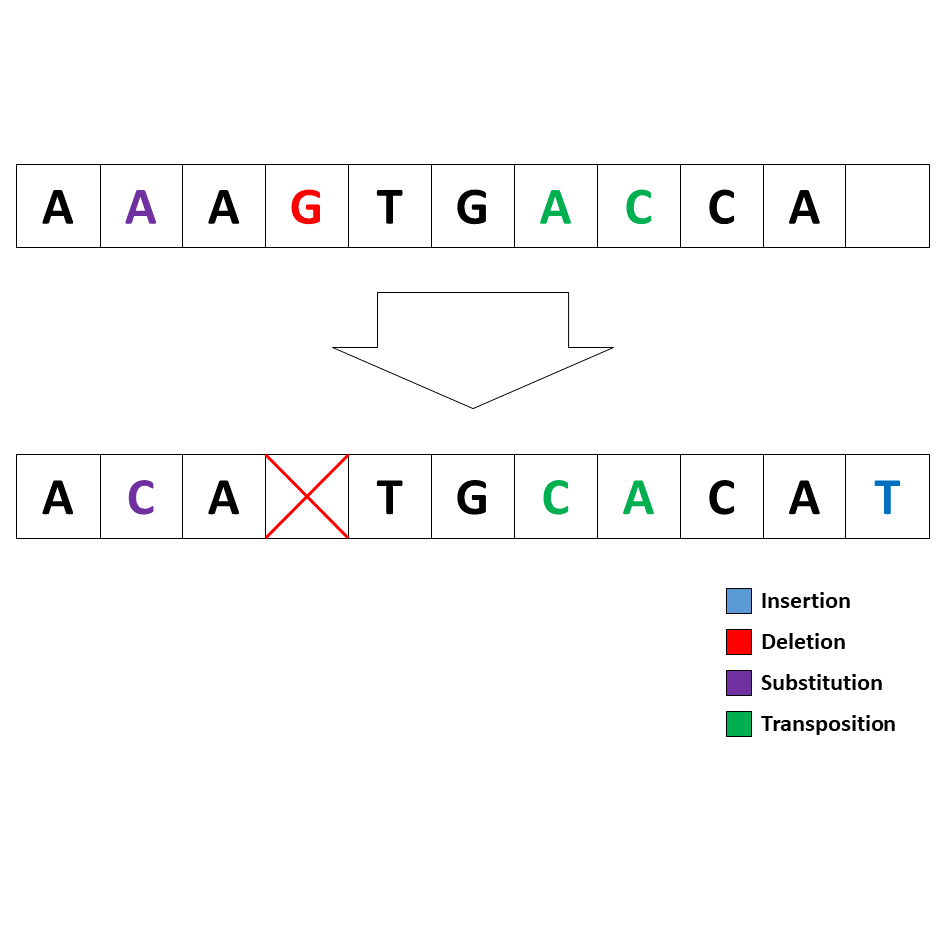
\includegraphics[width=0.75\textwidth]{figures/Graphics/Slide6.PNG}
    \caption{Shows two sequences. The edit distance is the sum of multiple operations. Blue shows an insert, red a deletion, purple a substitution and green a transposition. Therefore the edit distance is 4.}
    \label{fig:dl_example}
\end{figure}


\noindent In \autoref{eq:damerau_levenshstein} depicts the recursive formulation of the distance. The distance computes the costs of transforming the sequence $a$ to $b$, by computing the minimum of five seperate terms.  
% TODO: change a to e for consistency with model formulation
% TODO: Read on sequence alignment literature. Also add the readup to the literature review.
\begin{align}
    \label{eq:damerau_levenshstein}
    d_{a, b}(i, j) & =\min
    \begin{cases}
        \editDistance{i-1}{j  }+ 1 & \text { if } i>0                                            \\
        \editDistance{i  }{j-1}+ 1 & \text { if } j>0                                            \\
        \editDistance{i-1}{j-1}+ 1 & \text { if } i, j>0                                         \\
        \editDistance{i-2}{j-2}+ 1 & \text { if } i, j>1 \land a_{i}=b_{j-1} \land a_{i-1}=b_{j} \\
        0                                 & \text { if } i=j=0                                         
    \end{cases}        
\end{align}

\noindent The recursive form $d_{a, b}(i, j)$ for sequences $a$ and $b$ with respective elements $i$ and $j$ takes the minimum of each of each allowed edit operation. In particular, no change, deletion, insertion, substitution and transposition. For each operation, the algorithm adds an edit cost of 1. For Process Mining, it becomes necessary to modify the distance further. 

% TODO: Change a, b and c to x, y and z or e_1, e_2 and e_3
To illustrate the issue, we explore a couple of examples. Lets assume, we have two strings $s^1=aaba$ and $s^2=acba$. Using the Damerau-Levenshtein-Distance, the edit distance between both sequences is zero, as we can recognise one substitution at the second character in both strings. However, this representation is insufficient for process instances as they may also contain attibute values. Therefore, we characterise the sequences as process events in \autoref{eq:dlexample}. 

\begin{align}
    \label{eq:dlexample}
    s^1 &=\{a,a,b,a\} \\
    s^2 &=\{a,a^*,b,a\}\\
    s^3 &=\{a,c,b,a\}\\
    s^4 &=\{a,b,a\}
    &a,b,c \in \mathbb{R}^3\\
    a &= \begin{bmatrix}
        2\\
        1\\
        4\\
    \end{bmatrix}
    a^* = \begin{bmatrix}
        3\\
        3\\
        4\\
    \end{bmatrix}
    b = \begin{bmatrix}
        1\\
        1\\
        0\\
    \end{bmatrix}
    c = \begin{bmatrix}
        3\\
        1\\
        4\\
    \end{bmatrix}
\end{align}

\noindent If we do not consider attribute values, it becomes clear that $s^2$, $s^3$ and $s^4$ have an edit distance of 0, 1 and 1 to $s^1$. However, with attribute values $s^1$ and $s^2$ display clear differences. Similarly, $s^1$ and $s^3$ not only differ in terms of activity but also attribute value. Lastly, $s^1$ and $s^4$ are the same in attribute values, but one element still misses entirely. These examples show that we can neither disregard attribute values nor events, while computing the edit distance of two \glspl{instance}. 
We show this in \autoref{fig:image_with_dl}. 
In other words, we cannot simply assume a static cost of 1 for each edit operation. Instead, we have to define a cost function which takes attribute variables into account. In the following sections, we will establish distances which use a modified \gls{damerau_levenshtein} approach. Here, the cost of each edit-operation will be weighted with a distance function that considers the difference between event attributes. In simplified terms, we can say that $s^1$ and $s^2$ are identical, if we only consider the activity. However, taking attribute values into account, $s^1$ and $s^2$ actually differ on two accounts. 

% \begin{figure}[htb]
%     \centering
%     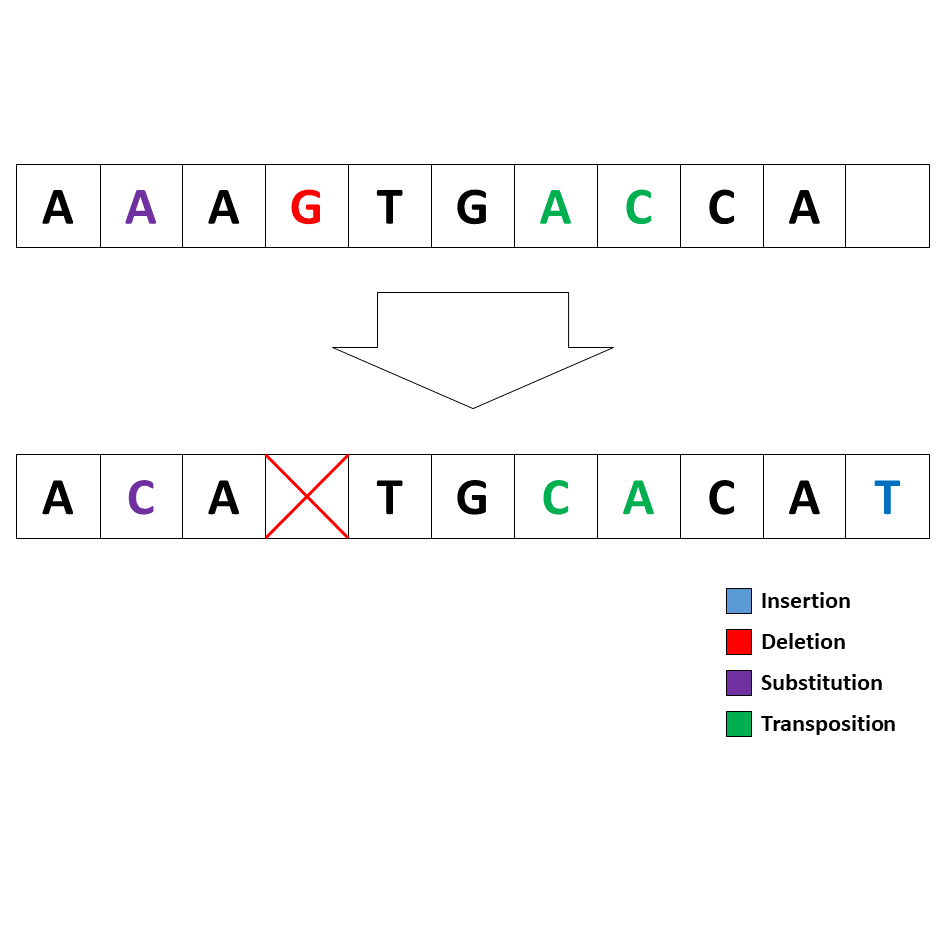
\includegraphics[width=0.99\textwidth]{figures/Graphics/Slide6.PNG}
%     \caption{This figure exemplifies the differeneces between the normal DL-distance and this one used.}
%     \label{fig:image_with_dl}
% \end{figure}

% \needsfigure{fig:image_with_dl}{This figure exemplifies the differeneces between the normal DL-distance and this one used.}

\noindent In order to reflect these differences in attribute values, we introduce a modified version of the \gls{damerau_levenshtein}, that not only reflects the difference between two process instances, but also the attribute values. We achieve this by introducing a cost function $\editCost$, which applies to a normed vector-space\footnotemark. Concretely, we formulate the modified \gls{damerau_levenshtein} as shown in \autoref{eq:modified_dl}. For the remainder, we will denote this edit-distance as \gls{SSDLD}.\footnotetext{A normed vector-space is a vector space, in which all vectors have the same dimensionality. For instance, if all vectors have three dimensions, we can call the vector-space \emph{normed}.}
% TODO: Introduce a with a dash above to compare activities instead of the vector
% Make zero thicker to indicate a null vector
\begin{align}
    \label{eq:modified_dl}
    d_{a, b}(i, j) & =\min
    \begin{cases}
        \editDistance{i-1}{j  }+\editCostFunctionNoA & \text { if } i>0                                            \\
        \editDistance{i  }{j-1}+\editCostFunctionNoB & \text { if } j>0                                            \\
        \editDistance{i-1}{j-1}+\editCostFunctionBoth & \text { if } i, j>0   \\ & \text { \& } \overline{a}_i=\overline{b}_j                                       \\
        \editDistance{i-1}{j-1}+ \editCostFunctionNoB +\editCostFunctionNoA  & \text { if } i, j>0  \\ & \text { \& } \overline{a}_i \neq \overline{b}_j                                       \\
        \editDistance{i-2}{j-2}+\editCostFunction{a_i}{b_{j-1}} + \editCostFunction{a_{i-1}}{b_j} & \text { if } i, j>1 \\ 
        & \text { \& } \overline{a}_i=\overline{b}_{j-1} \\ 
        & \text { \& } \overline{a}_{i-1}=\overline{b}_j \\
        0                                 & \text { \& } i=j=0                                          
    \end{cases} 
\end{align}

\noindent Here, $d_{a, b}(i, j)$ is the recursive form of the Damerau-Levenshtein-Distance. $a$ and $b$ are sequences and $i$ and $j$ specific elements of the sequence. $cost(a,b)$ is a cost function which takes the attribute values of $a$ and $b$ into account. 
The first two terms correspond to a deletion and an insertion from $a$ to $b$. The idea is to compute the maximal cost for that the wrongfully deleted or inserted event. 
The third term adds the difference between two events with identical activities $\overline{a}_i$ and $\overline{b}_j$. As mentioned earlier, two events that refer to the same activity can still be different due to event attributes. The distance between the event attributes determines \emph{how} different these events are. 
The fourth term handles the substitution of two events. Here, we compute the substitution cost as the sum of an insertion and a deletion. 
The fifth term computes the cost after transposing both events. This cost is similar to term 3 only that we now consider the differences between both events after they were aligned. The last term relates to the stopping criterion of the recursive formulation of the \gls{damerau_levenshtein}.  


\subsection{Discussing the Semi-Structured DL Distance}
There are two important characteristics, which require a discussion.

First, if we assess the first two terms, we use $cost(x,0)$ to denote the maximal distance of inserting and deleting x. $cost(x,0)$ can be read as cost between $x$ and a null-vector of the same size. However, it is noteworthy to state that this interpretration does not hold for any arbitrary cost-function. For instance, the cosine-distance does not work with a null vector, as it is impossible to compute the angle between x and a null vector. Here, the maximum distance would just amount to 1. In contrast, the family of \Gls{minkowski} works well with this notion, because they compute a distance between two points and not two directions. 

Second, to explain the intuition behind most terms, it is necessary to establish a common understanding between the relationship of an event with its event attributes. Generally, we can have two notions of this relationship. 

For the first relationship, we consider the event and its attributes as seperate entities. This notion is reasonable, as some attributes remain static throughout the whole process run. If we take a loan application process as an example, an applicant's ethnic background will not change regardless of the event. This characteristic can be considered a case attribute, which remains static throughout the process run. This understanding would require us to modify the cost functions, as they treat the activity independently from its attribute values. In other words, if the activities of two events are $\overline{a}$ and $\overline{b}$, but their attribute values are $\left(\begin{smallmatrix}2 \\ 3\end{smallmatrix}\right)$ and $\left(\begin{smallmatrix}2 \\ 3\end{smallmatrix}\right)$, these events may be seen as more similar than two $\overline{a}$ and $\overline{a}$ with attribute values $\left(\begin{smallmatrix}2 \\ 3\end{smallmatrix}\right)$ and $\left(\begin{smallmatrix}5 \\ 0\end{smallmatrix}\right)$. 

A second notion would treat each event as an independent and atomic point in time. Hence, $a$ and $b$ would be considered completely different even if their event attributes are the same. This understanding is also a valid proposition, as you could argue that an event which occurs at nighttime is not the same event as an event at daytime. Here, the time domain is the main driver of distinction and the content remains a secondary actor. 

All the terms described in the \gls{SSDLD} follow the second notion. There are two reasons for this decision. First, treating event activities and event attributes seperately would further complicate the \gls{SSDLD}, as we would have to expand the cost structure. Second, the unmodified \gls{damerau_levenshtein} applies to discrete sequences, such as textual data with atomic words or characters. By treating each event as an discrete sequence element, we remain faithful to the original function.

\attention{Cahnge to a more consistent order of introducing the measures.}
\subsection{Delta-Measure}
% TODO: Change likelihood to delta
% TODO: Discuss the theoretical limits (value goes from -0.5 to 1) 
For this measure, we can evaluate the precision of a counterfactual trace by determining whether a counterfactual would lead to the desired outcome. For this purpose, we use the predictive model, which will out put a prediction base on the counterfactual sequence. However, it is often difficult to force a deterministic model to produce a different result. We can relax the condition by maximising the likelihood of the counterfactual outcome. If we compare the likelihood of the desired outcome under the factual sequence with the counterfactual sequence, we can determine an increase or decrease. Ideally, we want to increase the likelihood. We can compute the odds or the difference between the two likelihoods. We choose to use the delta.
\attention{Mention that Delta is a replacement name to avoid confusion.}
% TODO: \attention{Needs some thought or testing. Odds may  be too aggressive.}. In \autoref{eq:likelihood}, we define the function.

\begin{align}
    \label{eq:likelihood_measure}
    improvement = p(o^*|a^*)-p(o^*|a)
\end{align}

\noindent Here, $p(o|a)$ describes the probability of an outcome, given a sequence of events.\attention{Describe the more complicated view on this measure}

% TODO: Discuss how this formulation favors shorter sequences. Might be solved by using an exact sequence prob computation. Deep-Normalizing-Flows with VAE for instance.
% TODO: Discuss several options here: That we can use only likelihood or likelihood improvement. That using odds is too aggressive. That difference is better. And which to choose. BUT just using likelihood is similar too feasibility.

\subsection{Feasibility-Measure}
To determine the feasibility of a counterfactual trace, it is important to recognise two components. First, we have to compute the probability of the sequence of events themselves. This is a difficult task, given the \emph{open world assumption}. In theory, we cannot know whether any event \emph{can} follow after a nother event or not. However, we can assume that the data is representative of the process dynamics. Hence, we can simply compute the first-order transition probability by counting each transition. However, the issue remains that longer sequences tend to have a zero probability if they have never been seen in the data. 
% We use the Kneser-Ney Smoothing\autocite{chen_empiricalstudysmoothing_1999} approach to ensure that unseen sequences are accounted for.
Second, we have to compute the feasibility of the individual feature values given the sequence. We can relax the computation of this probability using the \emph{markov assumption}. In other words, we assume that each event vector depends on the current activity, but none of the previous events and features. Meaning, we can model density estimators for every event and use them to determine the likelihood of a set of features. Hence, we compute the joint probability of a case by using the forward algorithm\needscite{forward algorithm}. In \autoref{eq:feasibility_measure} shows the formulation. 

\begin{align}
    \label{eq:feasibility_measure}
    feasibility_e & =p(a_i|a_{i-1} \ldots a_1, \theta) \approx  p(a_i|a_{i-1}, \theta) \nonumber\\ 
    feasibility_f & =p(f_i|a_i, \theta) \nonumber\\
    feasibility & = \prod_{i=1}^{n}\left[p(f_i|a_i, \theta) * p(a_i|a_{i-1}, \theta)\right] 
    % TODO: Better naming for the first two densities. Transistion and Emission probs. 
    % TODO: Check formulation https://en.wikipedia.org/wiki/Hidden_Markov_model#Inference and align the formulars
    % TODO: Check formulation https://en.wikipedia.org/wiki/Forward_algorithm and align the formulars
    % TODO: Check https://en.wikipedia.org/wiki/Forward_algorithm and decide whether to use forward backward
\end{align}

\noindent Here, $a \text{ and } f$ are the activity and features of a particular event. Likewise, $\theta$ is the data sample which is used to determine the parameters of the density function. The first equation shows the approximation based on the markov assumption. 
% TODO: Discuss how this formulation favors shorter sequences. Might be solved by using an exact sequence prob computation. Deep-Normalizing-Flows with VAE for instance.

\subsection{Similarity-Measure}
We use a function to compute the distance between the factual sequence and the counterfactual candidates. Here, a low distance corresponds to a small change. For reasons explained earlier (\autoref{sec:ssdld}), we want to take the structural distance and the feature distance into account. Henceforth, we will use the previously established \gls{SSDLD}. 
% This distance computes the costs associated with aligning two sequences by taking changes, inserts, deletes and transpositions of elements into account. Each of these alignment operations is typically associated with a cost of 1. This allows us to directly compute the structural difference between two sequences regardless of their lenghts. 
% Instead of computing a cost of 1 for every operation, we compute a cost of a distance between the feature vectors of each step. This cost fuction allows us to take not only the sequential differences into account but also feature differences. 
The similarity distance uses a cost function as specified in \autoref{eq:similarity_measure}.

\begin{align}
    \label{eq:similarity_measure}
    \editCostFunctionBoth      & = L2(a_i, b_j) \\
    a_i,b_j        & \in \mathbb{R}^d \nonumber
\end{align}

\noindent Here, $dist(x,y)$ is an arbitrary distance metric. $i \text{ and } j$ are the indidices of the sequence elements $a \text{ and } b$, respectively.

\subsection{Sparcity-Measure}
Sparsity refers to the number of changes between the factual and counterfactual sequence. We typically want to minimize the number of changes. However, sparcity is hard to measure, as we cannot easily count the changes. There are two reasons, why this is the case: First, the sequences that are compared can have varying lengths. Second, even if they were the same length, the events might not line up in such a way, that we can simply count the changes to a feature. Hence, to solve this issue, we use the previously established \gls{SSDLD}. The sparcity distance uses a cost function as specified in \autoref{eq:sparcity_measure}.

\begin{align}
    \label{eq:sparcity_measure}                          
    \editCostFunctionBoth      & = \sum_d \mathbb{I}(a_{id} = b_{jd})  \\ 
    a_i,b_j        & \in \mathbb{R}^d \nonumber 
\end{align}

\noindent Here, $\sum_d \mathbb{I}(a_{id} = b_{jd})$ is an indicator function, that is used to count the number of changes in a vector.


% TODO: Expand on global measures like Plausibility and Diversity
% \subsection{Diversity} 
% To measure the diversity of the generated counterfactual candidates, we are interested in the differences between all counterfactual candidates. Diversity can be understood as the inverse of the average similarity of all counterfactual candidate pairs. However, as we have to incoporate the sequential aspect of the counterfactuals, we need to compute the similarity across the whole sequence. We could use the Sparsity measure but the Damerau-Levenshtein measure is expensive to compute. Therefore, we simply align the candidates on their last step and pad the sequence with zeros. Hence, all sequences will have the length of the longest sequence. Hence, we compute the diversity as follows:

% \begin{align}
%     diversity  & = \frac{1}{\frac{1}{nt} \sum_{n}\sum_{t} sim(a_t^n, b_t^n)  }  
% \end{align}

% Here, \attention{explain variables}.

\subsection{Discussion}
Given the current viability function we can already determine the optimal counterfactual:
\begin{displayquote}
    The optimal counterfactual flips the strongly expected factual outcome of a model to a desired outcome, maintaining the same trajectory as the factual in terms of events, with minimal changes its event attributes, while remaining feasible according to the data.
\end{displayquote}

\noindent The elements that fulfill these criteria make up the pareto surface of this multi-valued viability function. If each of the values are scaled a range between 0 and 1, the theoretical ceiling is 4. This value is only possible if we can flip the outcome of a factual sequence without chaning it. As this is naturally impossible for deterministic model predictions, the viability has to be lower than 4. 

Furthermore, we can already postulate, that a viability of 2 is an important threshold. If we score the viability of a factual against itself, a normalised sparcity and similarity value have to at its maximal value of 1. In contrast, the improvement has to be 0. The feasibility is 0 depending on whether the factual was used to estimate the data distribution or not. \attention{With these observations in mind, we determine that any counterfactual with a viability of at least to is a considerable counterfactual.} 

\end{document}